\documentclass{article}
\usepackage{CJKutf8, indentfirst, graphicx, subfigure}
\begin{document}
\begin{CJK}{UTF8}{bsmi}
\title{硬體設計與實驗 Lab3 Report}
\author{104021219 鄭余玄}
\date{}
\maketitle
\section{實做過程}
aaa

\subsection{Block diagram}
\begin{figure*}[]
\centering{
\hfill
  \subfigure[]{ \label{fig:sub1}
    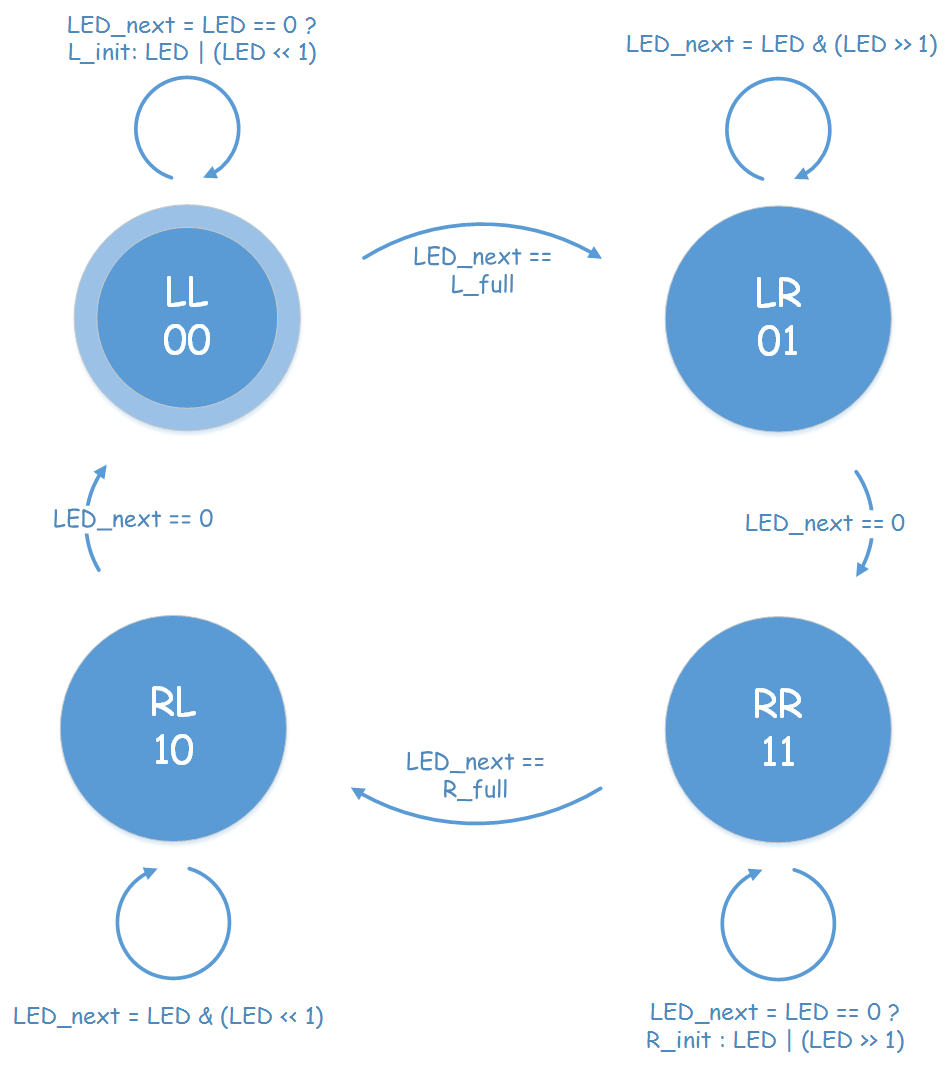
\includegraphics[width=.8\textwidth, angle=0]{lab3_1}
  }
\hfill
  \subfigure[]{ \label{fig:sub2}
    \includegraphics[width=.8\textwidth, angle=0]{lab3_2}
  }
}
\caption{Block diagrams: (a) lab3\_1 and (b) lab3\_2.}
\end{figure*}
aaa

\section{學到的東西及遇到的困難}
aaa

\section{想對老師或助教說的話}
aaa

\end{CJK}
\end{document}
